\section{Question 2}
Soit $A_{\Delta} = A + \Delta$ où $\Delta$ est une perturbation de moyenne nulle et d'écart-type 1. Le problème de départ $T_L X T_R = A_{\Delta}$ peut se décomposer en deux étapes \footnote{Si $A_{\Delta}$
est une matrice de dimension $n \times m$, $T_L$ (resp. $T_R$) sera une matrice carrée de dimension $n \times n$ (resp. $m \times m$).} :
\begin{eqnarray}
  \label{eq_q2}
  T_L \mathcal{Y} &=& A_{\Delta}\\
  T_R \mathcal{X}^T &=& \mathcal{Y}^T.
\end{eqnarray}
Qui en français correspond à résoudre le problème suivant : une photo a été flouté (on connait le type de floutage) puis une perturbation (inconnue) a dégradé la photo; et on souhaite déflouter la photo perturbé afin de retrouver l'image d'origine (la plus proche possible).



\subsection{Rayons spectraux}
Les matrices de Jacobi et de Gauss-Seidel sont définies comme suit :
\begin{eqnarray}
  \mathcal{J} &=& -D^{-1}(L+U)\\
  \mathcal{G} &=& -(D+L)^{-1}U,
\end{eqnarray}
autrement dit:
\begin{align*}
  \mathcal{J} & = - a
  \begin{bmatrix}
    1 & & &\\
      & 1 & &\\
      & & \ddots & \\
      & & & 1
  \end{bmatrix}
  \begin{bmatrix}
    0 & 1& &\\
    1 & \ddots & \ddots &\\
      & \ddots & \ddots & 1 \\
      & & 1 & 0
  \end{bmatrix}\\
  \mathcal{G} & = -
  \begin{bmatrix}
    1 & & &\\
    a & \ddots &  &\\
      & \ddots & \ddots  &  \\
      & & a & 1
  \end{bmatrix} ^{-1}
  \begin{bmatrix}
    0 & a & &\\
      & \ddots &  \ddots &\\
      &  & \ddots  & a \\
      & &  & 0
  \end{bmatrix}
  \\
  & = -
  \begin{bmatrix}
    1 & & & &\\
    -a & \ddots &  & &\\
    a^2 & \ddots & \ddots  &  &\\
    \vdots & \ddots & \ddots & \ddots & \\
    (-1)^{n-1}a^{n-1} & & a^2 & -a & 1
  \end{bmatrix}
  \begin{bmatrix}
    0 & a & &\\
      & \ddots &  \ddots &\\
      &  & \ddots  & a \\
      & &  & 0
  \end{bmatrix}\\
  & = -
  \begin{bmatrix}
    0 & a & & &\\
    0 & -a^2 & \ddots  & &\\
    \vdots & a^3 & \ddots & \ddots  &\\
    \vdots & \vdots & \ddots & \ddots  & a \\
    0 & (-1)^n a^n & & a^3 & -a^2
  \end{bmatrix}
\end{align*}

Pour la méthode de Jacobi, on obtient directement (cf. question 1) que les valeurs propres de $\mathcal{J}$ valent
$\lambda _i = -2a \cos(\dfrac{i \pi}{n+1})$ et donc $\rho(\mathcal{J}) = \max |\lambda_i| < 2a$.
Ainsi la méthode de Jacobi convergera pour des valeurs de $a \leq 0.5$.


\subsection{Comparaison Jacobi et Gauss-Seidel}
Le tableau qui dresse un bilan comparatif des méthodes de Jacobi et de Gauss-Seidel pour différentes valeurs de $a$ (les valeurs de $k$ étant calculées en fonction de $a$).
\footnote{Les codes des méthodes de Jacobi et Gauss-Seidel définissent une solution $x$
tel que $|x-x^*|<\epsilon$ où $x^*$ est la solution exacte et $\epsilon$ a été arbitrairement fixé à $0.00001$}
\begin{table}
  \centering
  \begin{tabular}{|l|l|l|l|l|}
    \hline
    \multirow{2}{*}{$a$} & \multicolumn{2}{l|}{Jacobi} & \multicolumn{2}{l|}{Gauss-Seidel}\\
    \cline{2-5}
        & $i_1$ & $i_2$ & $i_1$ & $i_2$\\
    \hline
    0.2 & 18    & 19    & 13    & 13\\
    \hline
    0.4 & 71    & 76    & 41    & 44\\
    \hline
    0.45& 147   & 163   & 81    & 90\\
    \hline
    0.5 & 500   & 500   & 500   & 500\\
    \hline
  \end{tabular}
  \caption{Nombre d'itération nécessaire pour déflouter pour différentes valeurs de $a$ (le défloutage abandonne à 500 itérations).
  $i_1$ est le nombre d'itérations pour le premier système et $i_2$ pour le deuxième.}
  \label{tab:iter}
\end{table}
On constate bien que la méthode de Gauss-Seidel converge plus rapidement que celle de Jacobi. De plus, comme prédit précédemment, la méthode de Jacobi et de Gauss-Seidel divergent pour des valeurs de $a \geq 0.5$



\subsection{Représentation des résultats en fonction de $a$}
La figure~\ref{fig:a2} représente les étapes successives de l'image qui part
de la figure~\ref{fig:a2original}; qui est ensuite floutée (figure~\ref{fig:a2blurred});
on lui ajoute du bruit (figure~\ref{fig:a2noise}) et on essaie de défloutée l'image obtenue pour
obtenir la figure~\ref{fig:a2unblurred}.
On remarque que la figure~\ref{fig:a2unblurred} est assez proche de l'originale, ce qui s'explique par la valeur de $a$ assez faible.

On remarque également que les bords de la figure~\ref{fig:a2blurred} et ~\ref{fig:a2noise}
sont noircies.
Cela est du au fait qu'ils sont le résultat de $x' = \frac{x + ay}{1 + 2a}$ où $x$ est le pixel de l'image originale et $y$ le pixel d'à côté.
Comme ils sont à côté, $x \approx y$ donc on a $x' \approx x \frac{1+a}{1+2a}$, on multiplie donc $x$ par une valeur plus petite que 1 ce qui noirci le pixel
car $0$ correspont à noir et 255 à blanc.
\begin{figure}
  \centering
  \begin{subfigure}[b]{0.45\textwidth}
    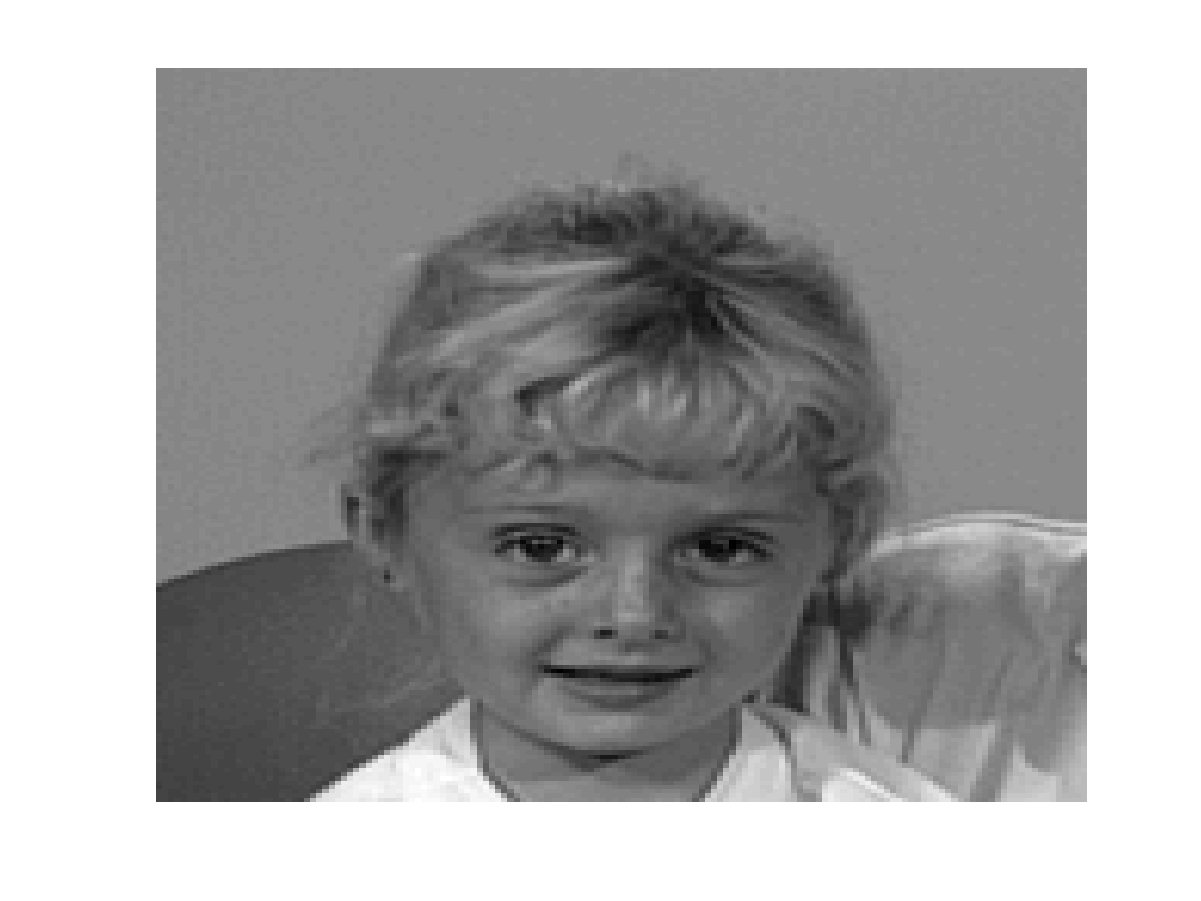
\includegraphics[width=\textwidth]{Q2/original_20.png}
    \caption{Image originale}
    \label{fig:a2original}
  \end{subfigure}%
  ~ %add desired spacing between images, e. g. ~, \quad, \qquad etc.
  %(or a blank line to force the subfigure onto a new line)
  \begin{subfigure}[b]{0.45\textwidth}
    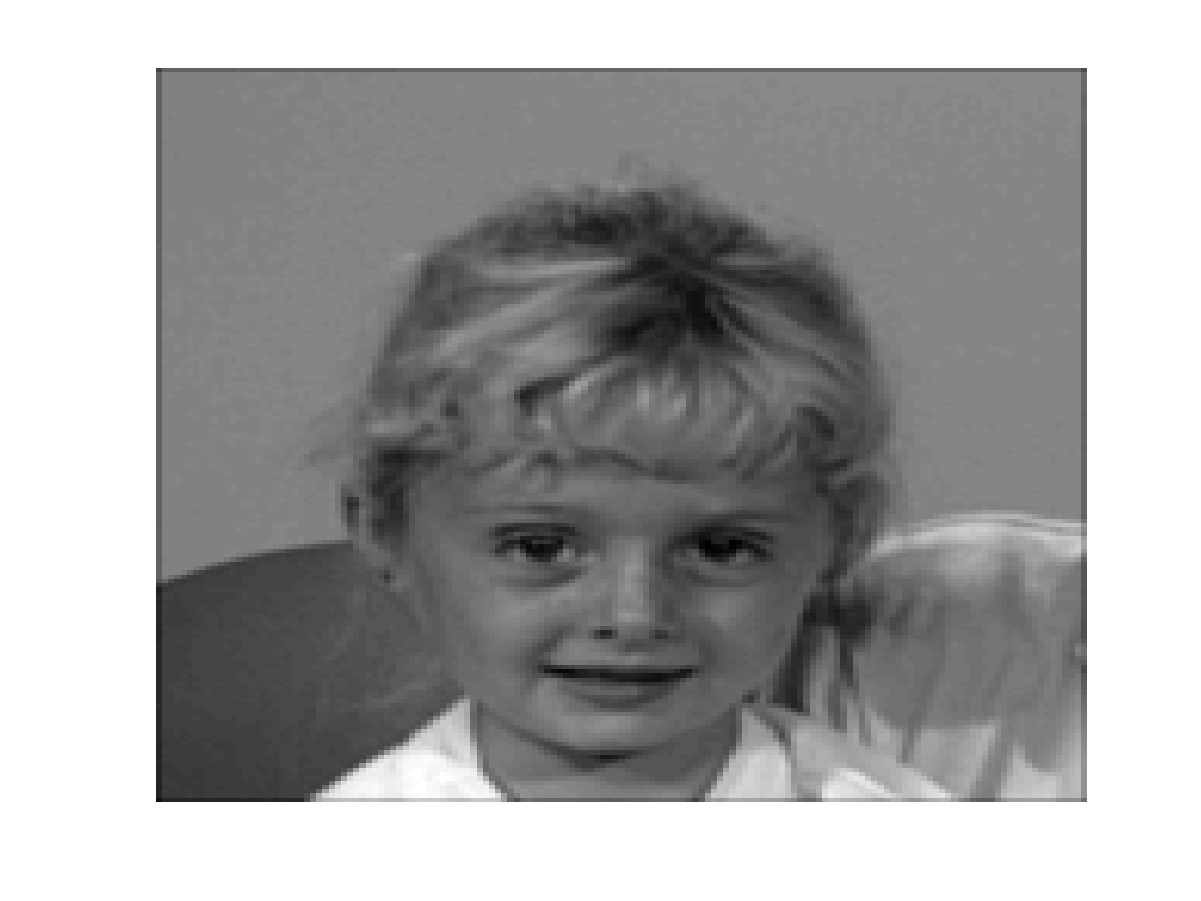
\includegraphics[width=\textwidth]{Q2/blurred_20.png}
    \caption{Image floutée}
    \label{fig:a2blurred}
  \end{subfigure}
  \begin{subfigure}[b]{0.45\textwidth}
    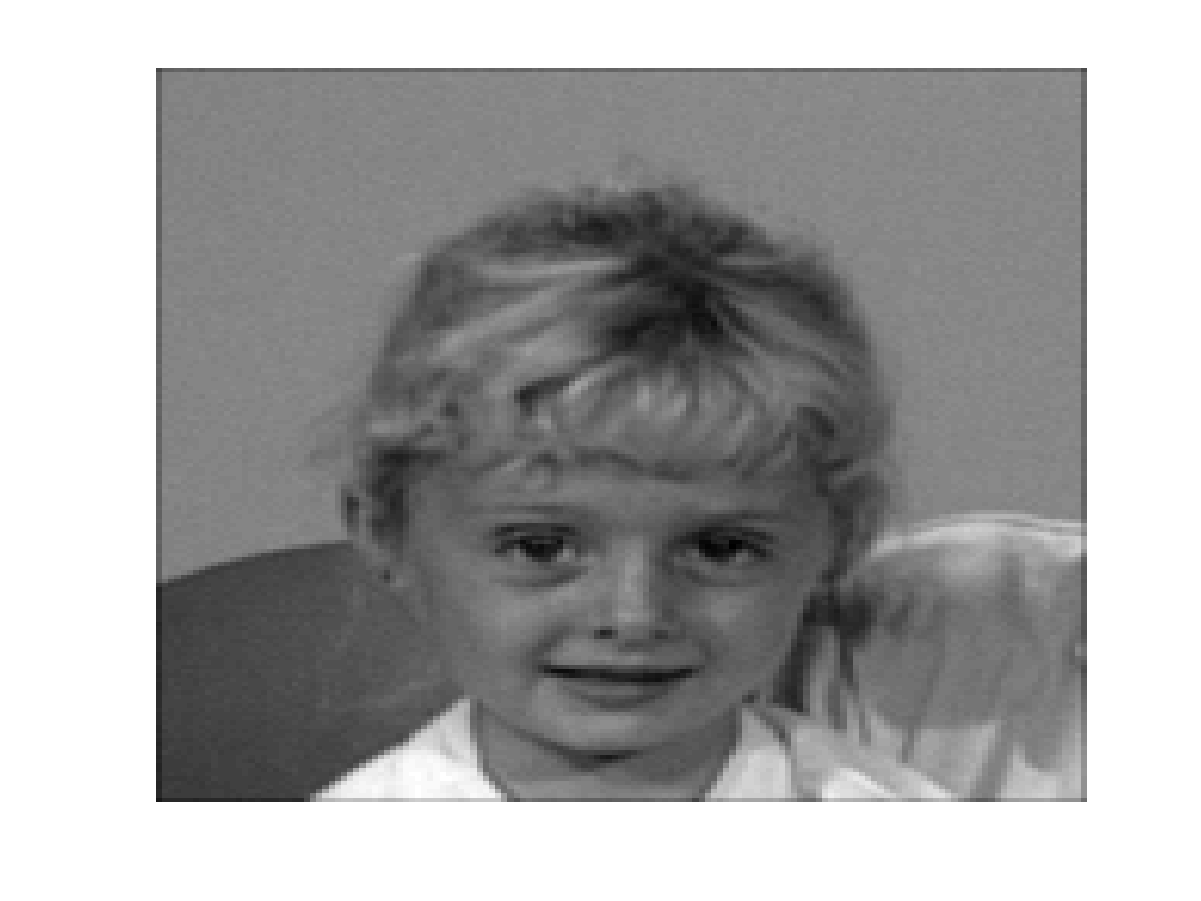
\includegraphics[width=\textwidth]{Q2/noise_20.png}
    \caption{Image floutée et bruitée}
    \label{fig:a2noise}
  \end{subfigure}%
  ~
  \begin{subfigure}[b]{0.45\textwidth}
    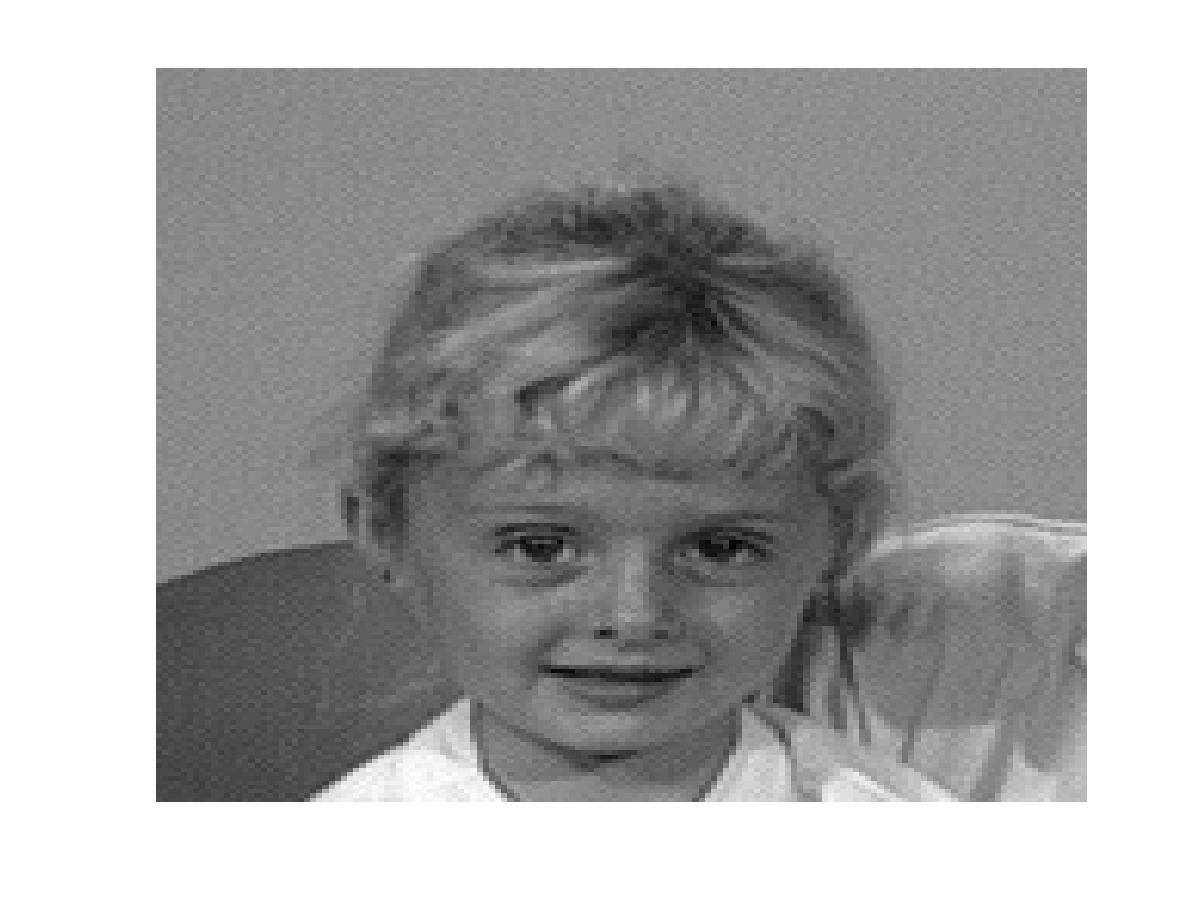
\includegraphics[width=\textwidth]{Q2/unblurred_20.png}
    \caption{Image floutée et bruitée défloutée}
    \label{fig:a2unblurred}
  \end{subfigure}
  \caption{Résultats pour $a = 0.2$}\label{fig:a2}
\end{figure}

La figure~\ref{fig:adiff} montre le résultat du défloutage pour différentes valeurs de $a$.
On a vu que plus $a$ était petit, plus vite on convergerait. De plus, à partir de $a = 0.5$, la convergence n'était plus assurée.
Ce qui est bien ce qu'on observe dans le tableau~\ref{tab:iter}, qui donne d'ailleurs un avantage
à Gauss-Seidel. 

On remarque aussi que
la figure~\ref{fig:a2unblurred} est meilleure que la figure~\ref{fig:a4} qui est meilleure
que la figure~\ref{fig:a45}.
La figure~\ref{fig:a5} ne ressemble plus du tout à la figure de départ et pour cause,
l'algorithme s'est arrêté après 500 itérations sans avoir convergé comme le montre
le tableau~\ref{tab:iter}.
Pourtant, le fait qu'on prenne plus de temps à converger ne veut pas dire qu'on arrive
pas à la solution voulue.
Cet effet est plutôt du au fait que lorsqu'on augmente $a$, le conditionnement de $T_L$
et $T_R$ s'éloignent de 1 se qui rend la résolution plus sensible au bruit.
% TODO, il faut vraiment analyser T_L et T_R ?? Non, plus M et N non ?

\begin{figure}
  \centering
  \begin{subfigure}[b]{0.3\textwidth}
    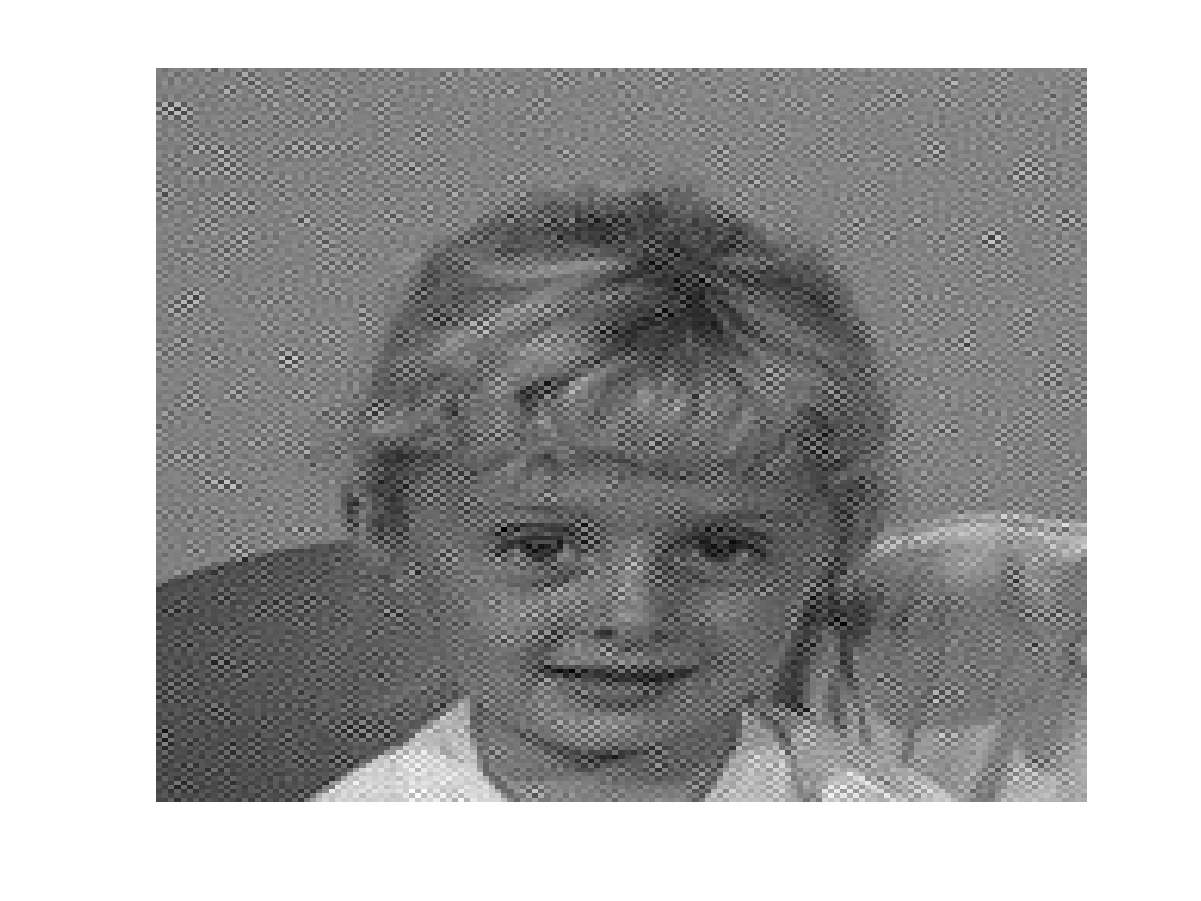
\includegraphics[width=\textwidth]{Q2/unblurred_40.png}
    \caption{$a = 0.4$}
    \label{fig:a4}
  \end{subfigure}%
  ~ %add desired spacing between images, e. g. ~, \quad, \qquad etc.
  %(or a blank line to force the subfigure onto a new line)
  \begin{subfigure}[b]{0.3\textwidth}
    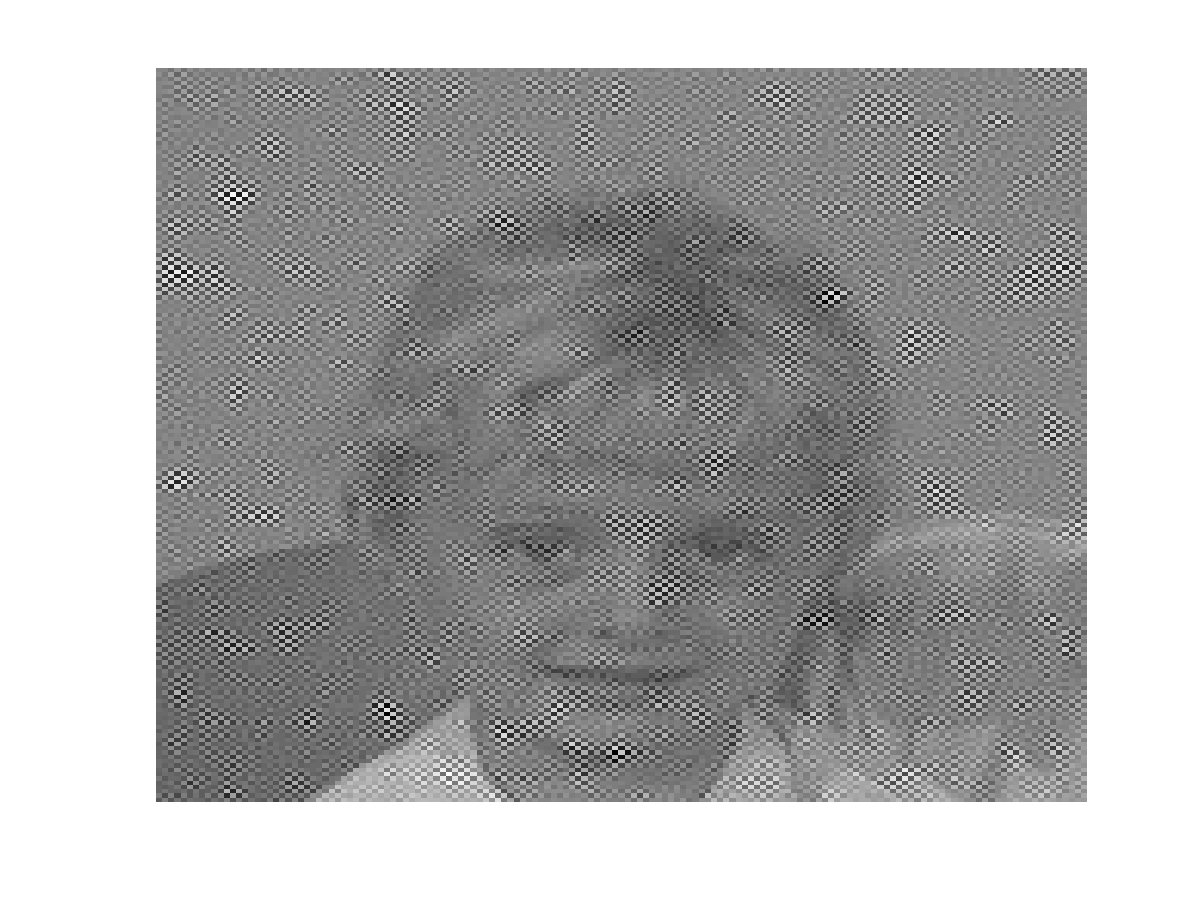
\includegraphics[width=\textwidth]{Q2/unblurred_45.png}
    \caption{$a = 45$}
    \label{fig:a45}
  \end{subfigure}%
  ~
  \begin{subfigure}[b]{0.3\textwidth}
    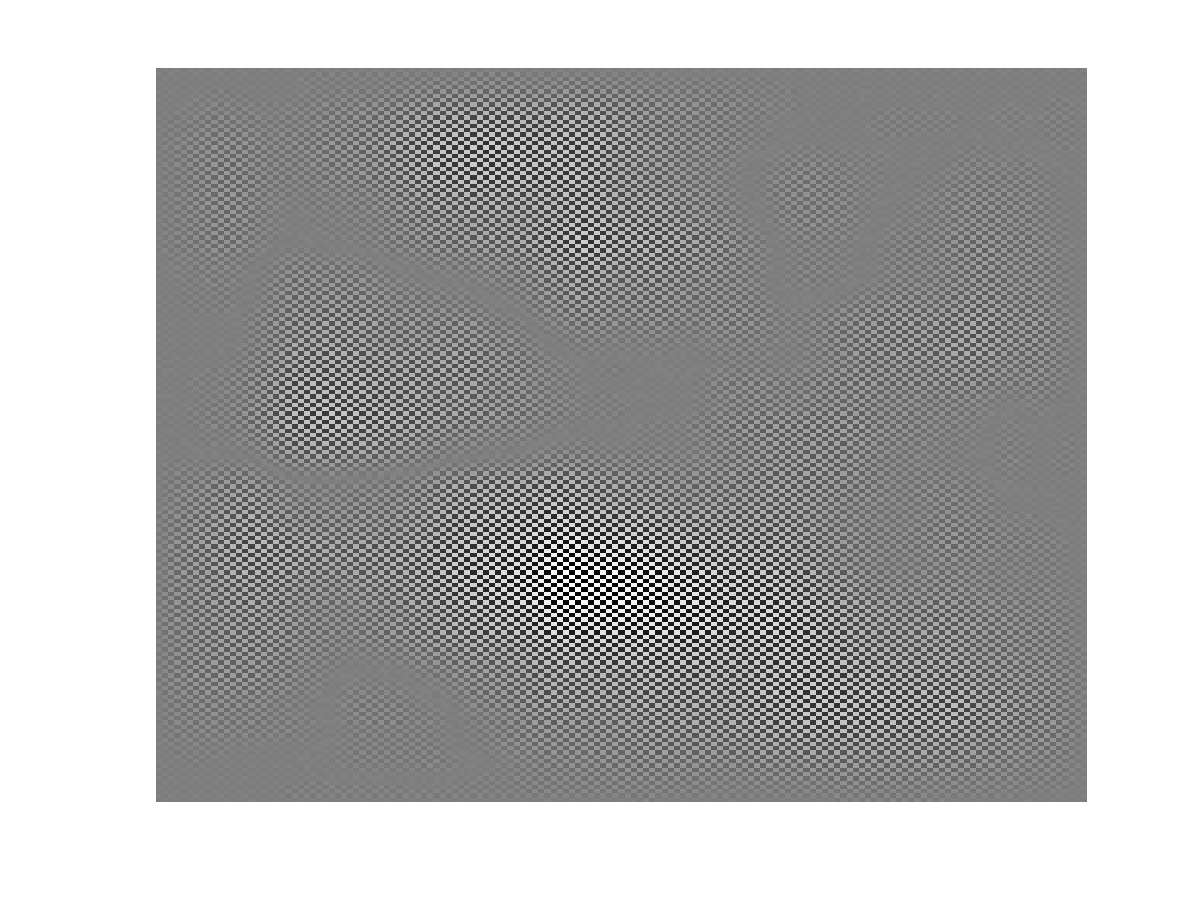
\includegraphics[width=\textwidth]{Q2/unblurred_50.png}
    \caption{$a = 0.5$}
    \label{fig:a5}
  \end{subfigure}
  \caption{Résultats du défloutage avec différentes valeurs de $a$}\label{fig:adiff}
\end{figure}



En effet, comme dit dans la question 1, le conditionnement $\kappa$ d'une matrice permet de donner une borne d'erreur de la solution si les conditions initiales dont entachées d'erreurs. Plus concrètement, si on cherche à résoudre le système linéaire $Ax=b$ et qu'on perturbe le vecteur $b\rightarrow b+\Delta b$, notre solution $x$ sera entachée d'erreur tel que : 
$$\frac{\Vert \Delta x \Vert}{\Vert x \Vert} \leq \kappa(A) \frac{\Vert \Delta b \Vert}{\Vert b \Vert} $$. 
Nous résolvons ici deux système successive (equations \ref{eq_q2}); et nous avons calculé dans la question 1 la valeur du conditionnent des matrices $T_L$ et $T_R$ (equation \ref{equatkappa}). Ce qui nous donne finalement : 
$$\frac{\Vert \Delta \mathcal{X} \Vert}{\Vert \mathcal{X} \Vert} \leq \kappa (T_R) \frac{\Vert \Delta \mathcal{Y} \Vert}{\Vert \mathcal{Y} \Vert} \leq \kappa(T_R) \kappa (T_L) \frac{\Vert \Delta \Vert}{\Vert A \Vert} = \left(\frac{1+2a}{1-2a}\right)^2  \frac{\Vert \Delta \Vert}{\Vert A \Vert}. $$
Où $\Delta$ est la perturbation de moyenne nulle et de variance 1 ajoutée à $A$. Numériquement cela nous donne \footnote{Les valeurs des perturbations relatives sont une moyenne sur 20 tests. Les normes matricielles utilisées sont des norme 2 implémenté sous Matlab dans la fonction \text{norm}} : 
\begin{eqnarray}
a=0.4  &\Longrightarrow & \kappa^2 = 81 \Longrightarrow 0.0366 \leq  0.1041\\
a=0.45  &\Longrightarrow & \kappa^2 = 361 \Longrightarrow  0.1242 \leq  0.4680\\
a=0.5  &\Longrightarrow &  \kappa^2 = \infty \Longrightarrow 1 \leq \infty 
\end{eqnarray}

Les résultats numérique confirme bien les prédictions théoriques













